\section{Эксперименты}\label{experiments}

Предлагаемый в данной работе метод протестирован с помощью открытого набора
данных OPT\cite{OPT}.
Эксперименты проводились на персональном компьютере с процессором Intel Core
i7CPU @ 2.7 GHz.
Данная работа исследует повышение точности трекинга, и наш алгоритм не работает
в режиме реального времени.
Поэтому сравнение различных модификаций алгоритма, а также сравнение с другими
алгоритмами проводится по точности трекинга.
Кроме того, различие в аппаратном обеспечении не позволяет корректно сравнивать
наш алгоритм с другими по производительности.

\subsection{Данные, используемые для тестирования}

OPT содержит шесть тестовых предметов, для каждого из которых отснято
по 92 видео с разрешением $1920\times1080$.
В каждом кадре известны истинные позиции объектов.
Предметы делятся на три группы по сложности геометрии 3D-моделей: простая
(Soda, Chest), средняя (Ironman, House) и высокая (Bike, Jet).

Видео записаны в различных условиях освещенности, воспроизводят разнообразные
траектории и скорости движения и поделены на следующие группы тестов:
\begin{itemize}
\item \term{$x$-$y$ translation} (\term{Tr}) "--- движение по окружности,
параллельной
        сенсору камеры.
\item \term{$z$ translation} (или \term{zoom}, \term{Zo}) "--- движение вперед
и
        назад вдоль оси, перпендикулярной сенсору камеры.
\item \term{In-plane rotation} (\term{Ir})"--- вращение вокруг оси,
перпендикулярной
        плоскости сенсора камеры.
\item \term{Out-of-plane rotation} (\term{Or})"--- вращение вокруг оси,
параллельной
        плоскости сенсора камеры.
\item \term{Flash light} (\term{Fl})"--- незначительное движение в мигающем
свете.
\item \term{Moving light} (\term{Ml})"--- незначительное движение объекта в
свете значительно
        перемещающегося источника освещения.
    \item \term{Free motion} (\term{Fm})"--- произвольное движение.
\end{itemize}

\Comment{Сокращения Fl, Ml, Tr и т. д. пока сюда написал. Возможно в 5.3 надо
перенести, но здесь они <<заодно>>}

Группы тестов \term{translation} и \term{rotation} содержат пять различных
уровней скорости.

\subsection{Измерение ошибки}

Ошибка оцененной позиции $\Pose_i$ в кадре $i$ вычисляется как
$
\delta_i = \avg_{\homv{x} \in \MeshV} \norm{\hat{\Pose_i} \homv{x} - \Pose_i
\homv{x}}
$,
где $\MeshV$~--- вершины 3D-модели,
а $\hat{\Pose_i}$ "--- истинная позиция объекта.
Положение объекта считается успешно найденным, если $\delta_i < k d$, где
$d$~--- максимальное из расстояний между всеми парами вершин, а $k$~---
заданный коэффициент ошибки.

Для оценки результатов трекинга строится кривая, каждая точка которой
определяется как процент кадров, на которых была успешно определена позиция
объекта, относительно варьируемого $k$.
Чем больше площадь под данной кривой (AUC), тем выше эффективность
рассматриваемого решения.
В данной работе берутся значения $k$ от 0 до 0.2.

\subsection{Анализ эффективности различных модификаций нашего метода}
Для сравнения между собой различных модификаций нашего алгоритма было собрано
подмножество датасета, включающее в себя наиболее часто встречающиеся на
практике паттерны движения.
К ним относятся произвольное движение, а также вращения и параллельные переносы
объекта относительно камеры на скорости $4$ (выше средней).
Эта скорость достаточно высокая, она приводит к небольшому смазыванию
изображений и встречается в реальных условиях.
При этом смазывание на ней ещё не слишком сильное и очертания объектов хорошо
различимы.
Также включены примеры с изменяющимся освещением, так как этот фактор негативно
влияет как на цветовой трекинг, так и на трекинг с использованием ключевых
точек.
Интерес здесь представляет исследование того, насколько комбинирование методов
помогает справляться с неблагоприятными условиями.

\subsubsection{Комбинирование методов}

Были протестированы метод на основе ключевых точек, метод на основе
распределения цвета и их комбинация.
На рис.~\ref{fig:combining-plots} представлены результаты трекинга этими
методами для разных групп тестов и для всего подмножества датасета.
В табл.~\ref{tab:combine} указаны значения AUC для соответствующих графиков.

\begin{table}[h]
\caption{\label{tab:combine}Результаты комбинирования методов в сравнении с
методами по отдельности}
\begin{center}
\begin{tabular}{|c|c|c|c|c|c|c|c|c|}
\hline
Метод & Общее & Fl & Fm & Ir & Ml & Or & Tr & Zo \\
\hline
Распределение цвета & 7.876 & $6.026$ & $7.757$ & $16.088$ & $5.471$ & $12.963$
&
$10.122$ & $3.743$ \\
\hline
Ключевые точки & 8.804 & $0.717$ & $8.561$ & $15.745$ & $11.248$ & $12.359$ &
$12.55$
&$12.219$ \\
\hline
Комбинация & $\mathbf{12.012}$ & $\mathbf{12.269}$ & $\mathbf{10.039}$ &
$\mathbf{16.932}$ &
$\mathbf{13.345}$ & $\mathbf{12.974}$ & $\mathbf{12.958}$ &
$\mathbf{12.583}$ \\
\hline
\end{tabular}
\end{center}
\end{table}

\begin{figure}
\centering
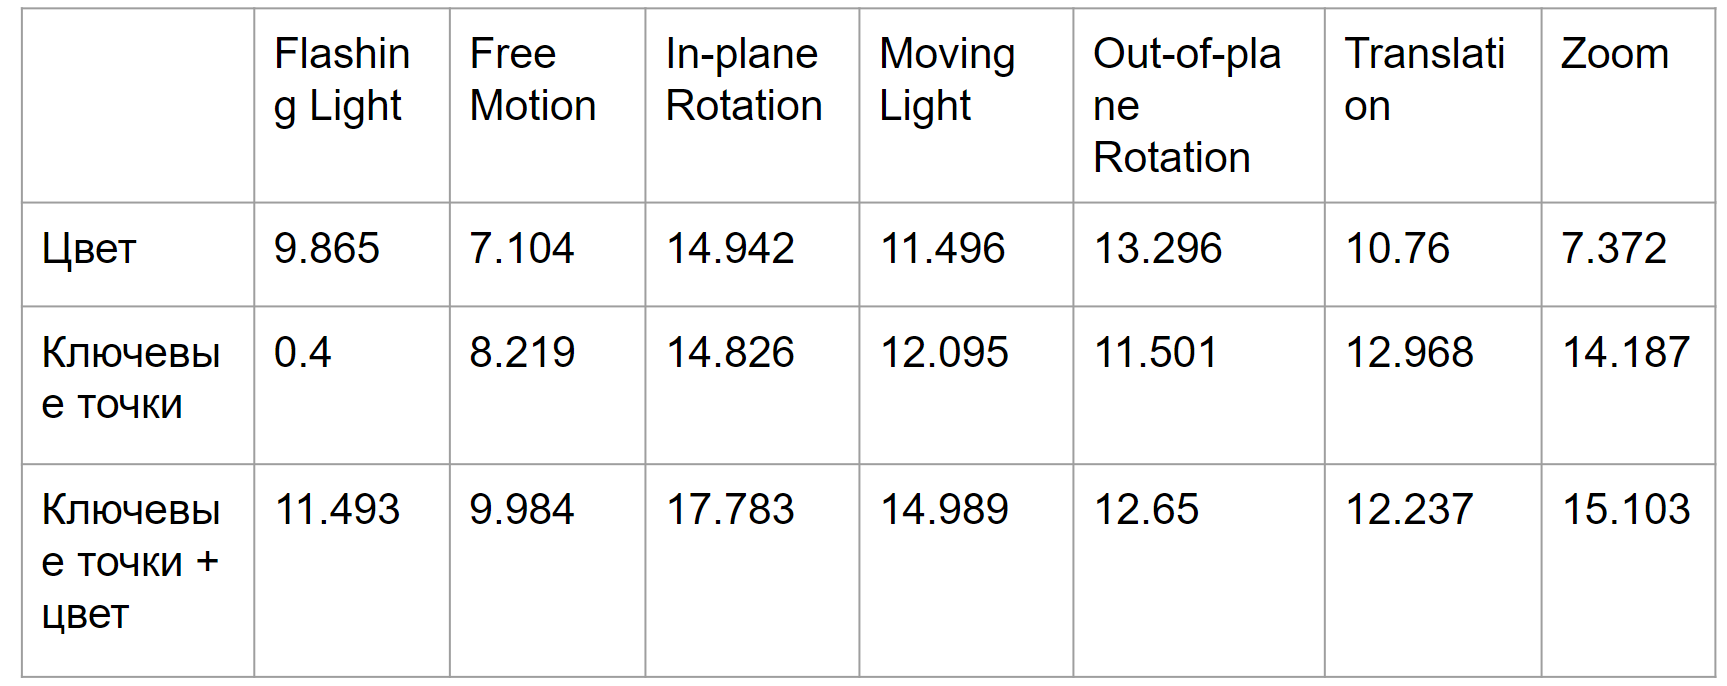
\includegraphics[width=0.9\textwidth]{fig/combining.pdf}
\caption{
Сравнение точности методов по отдельности и их комбинации на всём подмножестве
датасета и на группах тестов
}
\label{fig:combining-plots}
\end{figure}

\Comment{TODO: Заменить в таблице сокращения на полные названия или объяснить
сокращения}

Для всех групп комбинированный метод оказался лучше методов по отдельности.
По графику для всего подмножества датасета на рис.~\ref{fig:combining-plots}
можно заметить, что кривая для комбинированного метода почти совпадает с
кривыми для отдельных методов на левом конце и заметно превышает их на правом
конце графика.
Это говорит о том, что при комбинировании не увеличивается количество кадров,
где объект отслеживается почти идеально, но значительно растёт число кадров, на
которых объект отслеживается хотя бы с какой-то приемлемой точностью.

Комбинированный метод точнее отслеживает объект там, где отдельные методы
ошибались слишком сильно.
Таким образом, преимущества комбинирования более явно прослеживаются в сложных
для трекинга условиях.
Инициализация алгоритмом ключевых точек может значительно улучшить точность
цветового метода, что видно на примере группы \term{zoom}.
Это можно объяснить тем, что цветовой метод инициализируется вблизи глобального
минимума функции энергии, и даже если оптимизация сойдётся к локальному
минимуму, то результат будет недалёк от истинной позиции.

В группе тестов с мигающим светом (\term{Flash light}) оба отдельных метода
испытывают сложности, однако в комбинации удерживают друг друга вблизи
истинной позиции.
Позиция, уточнённая цветовым алгоритмом, помогает отфильтровать неправильно
отслеженные 2D-3D-соответствия.
Для ключевых точек, обнаруженных на кадре впервые, строятся более качественные
3D-прообразы.
Если эти точки будут прослеживаться хотя бы на нескольких кадрах, это во многих
случаях позволит строить по ним хорошую инициализацию цветового алгоритма.
Такая инициализация, в свою очередь, позволяет оптимиации сойтись гораздо ближе
к истиной позиции.

На группах тестов, где результаты отдельных методов не ниже $10$
(\term{In-plane rotation}, \term{Out-of-plane rotation}, \term{$x$-$y$
translation}), комбинация показывает незначительное улучшение, и её результат
примерно соответствует результату лучшего из отдельных методов.
Это тесты с постоянным освещением, где траекотрией движения является вращение
или перенос.
На них единственным фактором, негативно влияющим на качество трекинга, является
высокая скорость, и, как следствие, смазанность изображений.
Оба метода сохраняют работоспособность в таких условиях, и дополнение одного
метода другим незначительно увеличивает точность.


\subsubsection{Организация гистограмм}

В данной работе вводится подход к организации гистограмм, ограничивающий их
количество константой.
В то же время это потенциально может ухудшить точность метода в сравнении с
подходом, в котором для каждой вершины используется пара гистограмм.
В табл.~\ref{tab:full_hist} сравниваются два способа реализации
комбинированного алгоритма: в одном из них гистограммы организованы согласно
описанию в главе~\ref{tracking}.
В другом испольузется подход, описанный в~\cite{Tjaden2017}
и~\cite{Tjaden2018}: пара гистограмм строится для каждой вершины и действует в
окрестности её проекции, если эта проекция оказалась вблизи контура.
При тестировании мы использовали гистограммы всех вершин, спроецированных рядом
с контуром, в отличие от~\cite{Tjaden2017} и~\cite{Tjaden2018}, где выбиралась
только часть таких вершин.
Это позволяет обновлять информацию в большем числе гистограмм и избавляет от
рисков, связанных с неправильным их выбором, хотя и ухудшает
производительность.

\begin{table}[h]
\caption{\label{tab:full_hist}Влияние организации гистограмм на точность}
\begin{center}
\begin{tabular}{|c|c|c|c|c|c|c|c|}
\hline
Метод & Fl & Fm & Ir & Ml & Or & Tr & Zo \\
\hline
Пара гистограмм на каждую вершину & $7.27$ & $\mathbf{11.126}$ &
$\mathbf{17.279}$ & $12.302$ & $\mathbf{15.279}$ & $12.529$ &
$\mathbf{13.723}$\\
\hline
32 пары гистограмм & $\mathbf{12.269}$ & $10.039$ & $16.932$ &
$\mathbf{13.345}$ & $12.974$ &
$\mathbf{12.958}$ & $12.583$ \\
\hline
\end{tabular}
\end{center}
\end{table}

Можно заметить, что на большинстве паттернов  точность не уменьшилась, либо
уменьшилась незначительно.
Заметно снижение точности на паттернах \term{Or} и \term{Fm}.
На них объект при движении поворачивается другой, не видимой ранее, стороной, и
начинают использоваться гистограммы, достаточная статистика по которым ещё не
собрана.
Менее плотное распределение гистограмм в этом случае ухудшает результат.

\Comment{Добавить результаты цветового метода?}

\subsubsection{Влияние пересчёта 3D-прообразов ключевых точек}

Позиция, полученная цветовым методом, используется для задания 3D-прообразов
ключевых точек, появившихся на текущем кадре впервые.
Вместе с тем, она используется и для коррекции старых точек, если эта коррекция
уменьшает ошибку репроекции.

Если не обновлять 3D-прообразы старых ключевых точек, то они вычисляются
единожды при первом появлении ключевой точки на видео.
Даже если этот прообраз был найден неточно, он в дальнейшем не обновляется.

В табл.~\ref{tab:reprojection} представлены результаты трекинга с коррекцией
старых 3D-позиций и того же алгоритма, в котором 3D-позиции вычисляются
только при первом появлении ключевой точки и далее не пересчитываются.

\begin{table}[h]
\caption{\label{tab:reprojection}Влияние пересчёта 3D-прообразов}
\begin{center}
\begin{tabular}{|c|c|c|c|c|c|c|c|}
\hline
Метод & Fl & Fm & Ir & Ml & Or & Tr & Zo \\
\hline
Вычисление 3D-позиций при первом появлении & $11.209$ & $8.651$ & $16.649$ &
$\mathbf{13.698}$ & $12.788$ & $\mathbf{12.975}$ &
$\mathbf{13.59}$ \\
\hline
С коррекцией старых точек & $\mathbf{12.269}$ & $\mathbf{10.039}$ &
$\mathbf{16.932}$ & $13.345$ &
$\mathbf{12.974}$ &
$12.958$ & $12.583$ \\
\hline
\end{tabular}
\end{center}
\end{table}

Коррекция 3D-позиций в ходе трекинга улучшает точность на группе \term{flash
light}, где алгоритм ключевых точек сам по себе работает плохо.
Также заметно улучшение на группе \term{free motion}, что можно объяснить
большим разбросом 3D-прообразов одной и той же точки, вычисленных на разных
кадрах.
Это увеличивает вероятность того, что первоначально вычисленный 3D-прообраз
оказался недостаточно точен, но можно будет найти лучший по следующим кадрам.

В группе \term{zoom} трекинг с коррекцией 3D-прообразов менее точен, чем с
однократным их вычислением.
Негативное влияние коррекции здесь может быть связано с 2D-точками, которые
стали отслеживаться неправильно.
Коррекция их 3D-прообразов приводит к тому, что и 3D-позиции смещаются
относительно своего первоначального положения.
<<Неправильное>> 2D-3D-соответствие согласуется, тем не менее, с последней
вычисленной позицией, так как было обновлено в соответствии с ней.
Без репроекции 3D-позиции такое соответствие было бы отфильтровано, и не
оказывало бы в дальнейшем негативного влияния на трекинг.
%На группе \term{zoom} цветовой трекинг менее точен, чем трекинг на ключевых
%точках.
%В ходе трекинга точность может ухудшаться, поэтому и обновление позиции по
%менее точным кадрам несколько ухудшает результаты.
%На остальных группах пересчёт позиций не улучшает качество трекинга, либо
%улучшает его незначительно.

\Comment{Объяснения пока очень предположительные}

\subsubsection{Сравнение с аналогами}

В табл.~\ref{tab:analogues} представлено сравнение предлагаемого алгоритма с
алгоритмами на основе распределения цвета (PWP3D, RBOT) и комбинированными
алгоритмами (Bugaev et.al., Zhong et.al.).

\begin{itemize}
\item PWP3D "--- один из первых цветовых алгоритмов, в котором использовалась
одна пара гистограмм для всего изображения.
\item RBOT "--- цветовой алгоритм с одной парой гистограмм для каждой вершины
объекта.
\item Bugaev et. al. "--- алгоритм, в котором совмещались трекинг на ключевых
точках с методом, основанным на контурах. Ключевые точки также использовались
для инициализации трекинга, а затем --- для задания ограничений при оптимизации
контурной функции ошибки.
\item Zhong et.al. "--- алгоритм, в котором отслеживается распределение цвета в
окрестностях контура и градиентные дескрипторы на внутренней части переднего
плана.
\end{itemize}

\begin{table}[h]
\caption{\label{tab:analogues}Сравнение с другими цветовыми и комбинированными
алгоритмами}
\begin{center}
\begin{tabular}{|c|c|c|c|c|c|c|c|}
\hline
Объект & Bike & Chest & House & Ironman & Jet & Soda & Среднее \\
\hline
PWP3D~\cite{PWP3D} & $5.358$ & $5.551$ & $3.575$ &
$3.915$ & $5.813$ & $5.87$ & $5.014$ \\
\hline
RBOT~\cite{Tjaden2018} & $11.903$ & $11.764$ & $10.15$ &
$11.986$ & $13.217$ & $8.861$ & $11.314$ \\
\hline
Bugaev et.al.~\cite{Bugaev_2018_ECCV} & $12.55$ & $14.97$ & $14.48$ &
$\mathbf{14.71}$ & $\mathbf{17.17}$ & $\mathbf{14.85}$ & $\mathbf{14.79}$ \\
\hline
Zhong et.al.~\cite{Zhong2020} & $\mathbf{12.831}$ & $12.24$ & $13.613$ &
$11.214$ & $15.441$ & $9.012$ & $12.392$ \\
\hline
Наш алгоритм & $11.648$ & $\mathbf{15.522}$ & $\mathbf{16.607}$ & $11.556$ &
$13.966$ & $14.104$
& $13.901$ \\
\hline
\end{tabular}
\end{center}
\end{table}

За счёт локальности RBOT и наш алгоритм работают значительно лучше PWP3D. 
Наш метод незначительно уступает RBOT на объектах Bike и Ironman. Эти объекты
имеют большое количество вершин, и RBOT может иметь преимущество за счёт
большего количества гистограмм. Тем не менее, благодаря использованию ключевых
точек, разница в точности получается небольшой. На хорошо текстурированных
объектах Chest и House инициализация цветового метода ключевыми точками
позволяет показать значительно превзойти результат RBOT.

На объектах более простой геометрии предложенный комбинированный метод
значительно превосходит RBOT.
Преимущества комбинирования явно прослеживаются на объекте Soda. 
Этот объект симметричен относительно оси вращения, и цветовой алгоритм
испытывает трудности при его трекинге.
Использование ключевых точек помогает разрешать неоднозначности, связанные с
одинаковым контуром при разных углах поворота объекта вокруг своей оси.

Можно заметить, что наш алгоритм превосходит аналоги на объектах Chest и House.
Это объекты невысокой полигональности с достаточным количеством ключевых точек
на текстуре.
На большей части объектов наш метод превосходит Zhong et.al., также применяющий
цветовую информацию для трекинга.
В том числе значительное улучшение отмечается на симметричном объекте Soda.
На объектах Chest и House предлагаемый метод показывает лучшие результаты, чем
алгоритм Bugaev et.al., но на некоторых объектах (Ironman, Jet) значительно
уступает.
Тем не менее, в среднем разница в точности не слишком большая.
Таким образом, в среднем алгоритм показывает результаты на уровне современных
комбинированных методов.

\Comment{TODO: больше алгоритмов для сравнения?}
\Comment{TODO: объяснение результатов в сравнении с Bugaev и Zhong?}
